\documentclass[../../../main.tex]{subfiles}

\begin{document}
\subsection*{Appendix I: Magnetic Forces}
\subsubsection*{Cyclotron motion.} A uniform magnetic field points into the page; if the charge $Q$ moves counterclockwise, with speed $v$, around a circle of radius $R$, the magnetic force points inward, and has a fixed magnitude $Qv B$—just right to sustain uniform circular motion:
\begin{align*}
    Qv B&=m\frac{v^2}{R}\\
    p&=QBR
\end{align*}
where $m$ is the particle’s mass and $p = mv$ is its momentum. 

\subsubsection*{Cycloid Motion.} Suppose, for instance, that $B$ points in the x-direction, and $E$ in the $z$-direction. A positive charge is released from the origin; what path will it follow?

There being no force in the x-direction, the position of the particle at any time t can be described by the vector $(0, y(t), z(t))$; the velocity is therefore
\begin{equation*}
    \mathbf{v} = \dot{y}\;\mathbf{\hat{y}}+ \dot{z}\;\mathbf{\hat{z}}
\end{equation*}
Thus
\begin{equation*}
    \mathbf{v}\times \mathbf{B}=\begin{vmatrix}
        \mathbf{\hat{x}}&\mathbf{\hat{y}}&\mathbf{\hat{z}}\\
        0& \dot{y}& \dot{z}\\
        B &0& 0\\
    \end{vmatrix}=
    B \dot{z}\mathbf{\hat{y}}-B\dot{y}\mathbf{\hat{z}}
\end{equation*}
applying Newton’s second law
\begin{align*}
    Q(\mathbf{E} + \mathbf{v} \times \mathbf{B}) &= m\mathbf{a}\\
    Q(B \dot{z}\mathbf{\hat{y}}+(E-B\dot{y})\mathbf{\hat{z}})&=m(\ddot{y}\mathbf{\hat{y}}+ \ddot{z}\mathbf{\hat{z}})
\end{align*}
Or, treating the $\mathbf{\hat{y}}$ and $\mathbf{\hat{z}}$ components separately
\begin{equation*}
    \ddot{y}=\omega \dot{z}\quad\text{and}\quad    \ddot{z}=\omega\biggl(\frac{E}{B}-\dot{y}\biggr)
\end{equation*}
where
\begin{equation*}
    \omega\equiv\frac{QB}{m}
\end{equation*}

To solve these differential equation, first I solve for $\ddot{z}$
\begin{equation*}
    \ddot{z}=\frac{1}{\omega}\dddot{y}=\omega\biggl(\frac{E}{B}-\dot{y}\biggr)
\end{equation*}
or 
\begin{equation*}
    \frac{d}{dt}\ddot{y}=\omega^2\biggl(\frac{E}{B}-\dot{y}\biggr)
\end{equation*}
Then I will do change of variable $\psi=\dot{y}$, thus
\begin{equation*}
    \ddot{\psi}+\omega^2\psi=\omega^2\frac{E}{B}
\end{equation*}
Reminder that the solution to differential equation is the superposition of its homogenous equation solution--called complementary-- and its particular solution. Its homogenous form is 
\begin{equation*}
    \ddot{\psi}+\omega^2\psi=0
\end{equation*}
which has the solution
\begin{equation*}
    \psi_c=\mathcal{A}\sin \omega t+\mathcal{B}\cos\omega t
\end{equation*}
For its particular solution, I shall rewrite the equation
\begin{align*}
    \ddot{\psi}+\omega^2\psi&=\omega^2\frac{E}{B}\\
    (D+\omega i)(D-\omega i)\psi&=e^{0\cdot t}\omega^2\frac{E}{B}
\end{align*}
which has the form of
\begin{equation*}
    (D+a)(D-b)y=e^{cx}P_n(x)
\end{equation*}
Since $c\neq a, c\neq b$ and $\omega^2E/B$ is polynomial of the zeroth degree, I have the particular solution
\begin{equation*}
    \psi_p=A
\end{equation*}
Substituting into my equation, I have
\begin{equation*}
    A=\frac{E}{B}
\end{equation*}
Then, my particular solution
\begin{equation*}
    \psi_p=\frac{E}{B}
\end{equation*}
And my total solution
\begin{equation*}
    \psi=\mathcal{A}\sin \omega t+\mathcal{B}\cos\omega t+\frac{E}{B}
\end{equation*}
Changing into my original variable, I have the solution of $y$
\begin{equation*}
    y=\mathcal{A}\cos \omega t+\mathcal{B}\sin\omega t+\frac{E}{B}t+\mathcal{D}
\end{equation*}

Substituting $y$ into
\begin{equation*}
    \ddot{y}=\omega \dot{z}
\end{equation*}
I have 
\begin{equation*}
    \mathcal{B}\cos \omega t- \mathcal{A}\sin \omega t=\omega \dot{z}
\end{equation*}
Thus, I have the solution for $z$
\begin{equation*}
    z=\mathcal{B}\cos \omega t-\mathcal{A}\sin \omega t+\mathcal{D}
\end{equation*}

Now, we apply the boundaries condition. We know that the particle started from rest $\dot{y}_0=\dot{z_0}=0$ at the origin $ y_0=z_0=0$. We have
\begin{align*}
    \begin{cases}
            y&=\mathcal{A}\cos \omega t+\mathcal{B}\sin\omega t+\frac{E}{B}t+\mathcal{D}\\
    \dot{y}&=\mathcal{B}\omega\sin\omega t-\mathcal{A}\omega\cos \omega t+\frac{E}{B}\\
    z&=\mathcal{B}\cos \omega t-\mathcal{A}\sin \omega t+\mathcal{D}\\
    \dot{z}&=-\mathcal{B}\omega\cos \omega t-\mathcal{A}\omega\sin \omega t
    \end{cases}
\end{align*}
applying the boundaries condition
\begin{align*}
    \begin{cases}
         \mathcal{A}+\mathcal{C}&=0\\
    \mathcal{B}&=-\frac{E}{B\omega}\\
    \mathcal{D}&=\frac{E}{B\omega}\\
    -\mathcal{A}\omega&=0
    \end{cases}
\end{align*}

Finally, I have 
\begin{equation*}
    y=\frac{E}{B\omega}(\omega t-\sin \omega t)\quad \text{and}\quad z=\frac{E}{B\omega}(1-\cos\omega t)
\end{equation*}

In this form, the answer is not terribly enlightening, but if we let
\begin{equation*}
    R\equiv\frac{E}{B\omega}
\end{equation*}
and eliminate the sines and cosines by exploiting the trigonometric identity, we find that
\begin{equation*}
    (y - R\omega t)^2 + (z - R)^2 = R^2
\end{equation*}
This is the formula for a circle, of radius $R$, whose center $(0, R\omega t, R)$ travels in the $y$-direction at a constant speed
\begin{equation*}
    u=\omega R=\frac{E}{B}
\end{equation*}

\subsection*{Appendix II: Biot-Savart's Law}

\subsubsection*{Straight Wire.} Find the magnetic field a distance s from a long straight wire  carrying a steady current $I$. 
\begin{figure*}[ht]
    \centering
    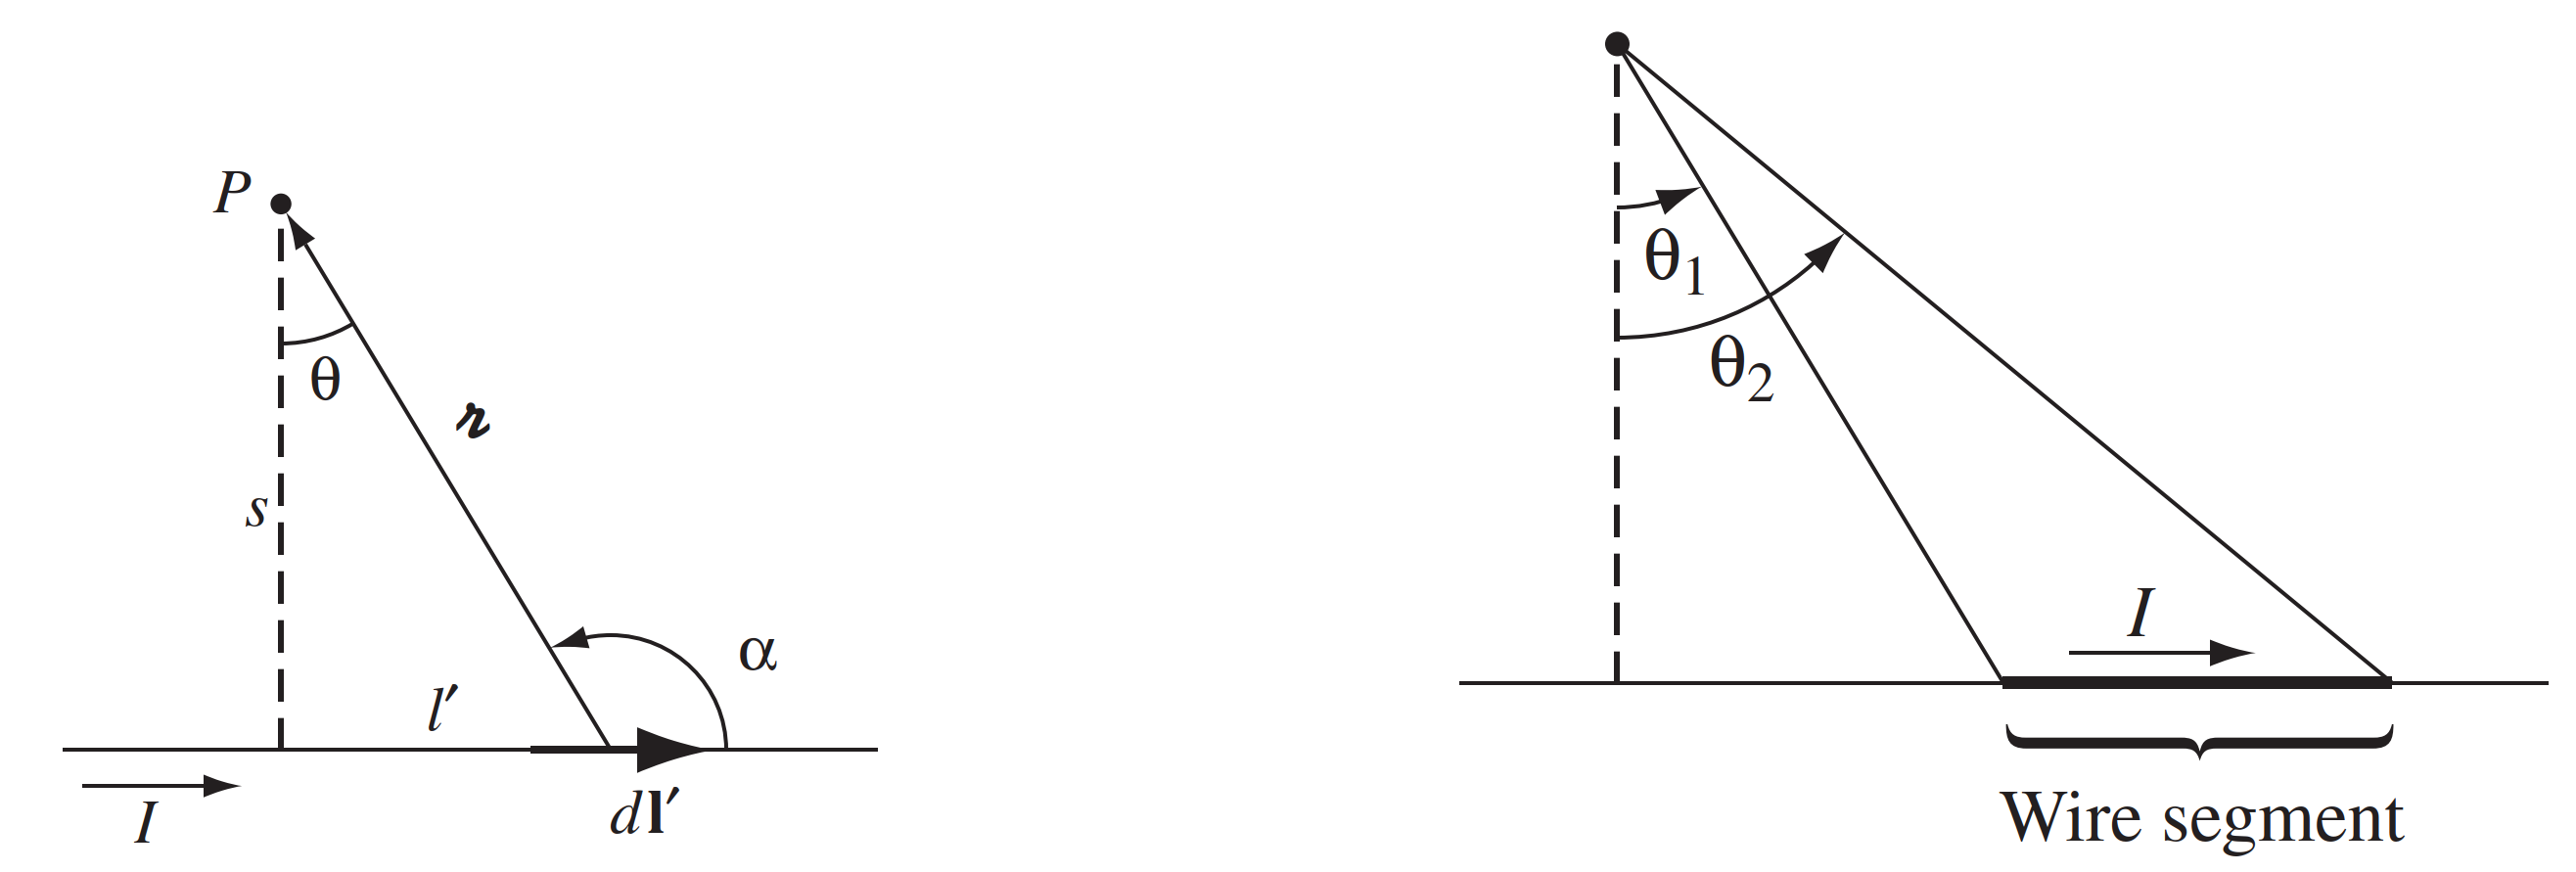
\includegraphics[width=0.7\textwidth]{../Rss/Electromagnetism/Magnetostatics/StraightWire.png}
\end{figure*}

I shall evaluate the magnetic field in cylindrical coordinate. I define the direction of current as the $z$ axis. Also, let's say that the length of the wire is $L$. First, we need to determine the separation vector
\begin{align*}
    \brcurs&=s\mathbf{\hat{s}}+z\mathbf{\hat{z}}\\
    |\rcurs|&=(s^2+z^2)^{1/2}
\end{align*}
Then, the magnetic field is
\begin{align*}
    \mathbf{B}& =\frac{\mu_0 I}{4\pi}\int \frac{d\mathbf{l}\times \brcurs}{|\rcurs^3|}\\
    \mathbf{B}&=\frac{\mu_0 I}{4\pi}\int \frac{(d s \;\mathbf{\hat{s}} +s \;d \phi \;\boldsymbol{\hat{\phi}}+  d z \;\mathbf{\hat{z}})\times(s\mathbf{\hat{s}}+z\mathbf{\hat{z}})}{(s^2+z^2)^{3/2}}\\
\end{align*}
since I'm only integrating along $z$, $ds=d\phi=0$
\begin{align*}
    \mathbf{B}&=\frac{\mu_0 I}{4\pi}\int_{-L/2}^{L/2} \frac{( dz \; \mathbf{\hat{z}}) \times (s\mathbf{\hat{s}}+z\mathbf{\hat{z}})}{(s^2+z^2)^{3/2}}\\
    \mathbf{B}&=\frac{\mu_0 I}{4\pi}\int_{-L/2}^{L/2} \frac{s\;dz}{(s^2+z^2)^{3/2}}\boldsymbol{\hat{\phi}}
\end{align*}
Evaluating the integral using trigonometric substitution
\begin{align*}
    \mathbf{B}&=\frac{\mu_0 I}{4\pi}s\frac{z}{s^2(s^2+z^2)^{1/2}}\bigg|_{-L/2}^{L/2}\boldsymbol{\hat{\phi}}\\
    \mathbf{B}&=\frac{\mu_0 I}{4\pi s}\frac{L}{(s^2+L^2/4)^{1/2}}\boldsymbol{\hat{\phi}}
\end{align*}
Or, in terms of the initial and final angles $ \theta_1$ and $\theta_2$
\begin{equation*}
    \mathbf{B}=\frac{\mu_0 I}{4\pi r}(\sin \theta_2-\sin\theta_1)\boldsymbol{\hat{\phi}}
\end{equation*}

In the case of an infinite wire, we integrate from $z=-\infty$ to $z=\infty$
\begin{align*}
    \mathbf{B}&=\frac{\mu_0 I}{4\pi}s\frac{z}{s^2(s^2+z^2)^{1/2}}\bigg|_{- \infty}^{\infty}\boldsymbol{\hat{\phi}}\\
    \mathbf{B}&=\frac{\mu_0 I}{2\pi s}\boldsymbol{\hat{\phi}}
\end{align*}

\subsubsection*{Two Straight Wire.}  Let’s find the force of attraction between two long, parallel 
wires a distance $d$ apart, carrying currents $I_1$ and $I_2$. The field at (2) due to (1) is
\begin{equation*}
    \mathbf{B}=\frac{\mu_0 I_1}{2\pi d}\boldsymbol{\hat{\phi}}
\end{equation*}
and it points into the page. The Lorentz force law predicts a force directed towards (1)
\begin{equation*}
    F=I_2\frac{\mu_0 I_1}{2\pi d}\int\;dl
\end{equation*}
The total force, not surprisingly, is infinite, but the force per unit length is
\begin{equation*}
    f=\frac{\mu_0 I_1I_2}{2\pi d}
\end{equation*}
If the currents are antiparallel (one up, one down), the force is repulsive.
\begin{figure*}[ht]
    \centering
    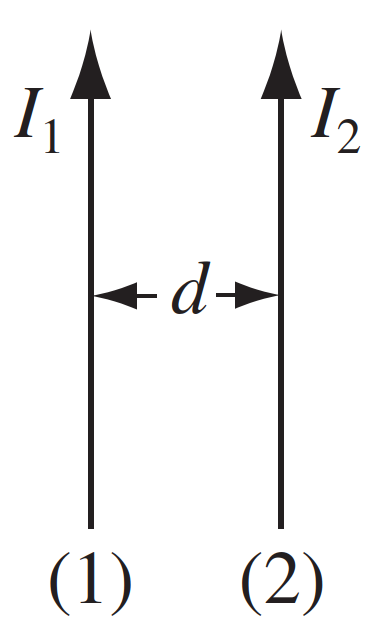
\includegraphics[height=0.3\textwidth]{../Rss/Electromagnetism/Magnetostatics/StraightWire2.png}
\end{figure*}


\subsubsection*{Loop.} Find the magnetic field a distance $z$ above the center of a circular loop of radius $R$, which carries a steady current $I$.
\begin{figure*}[ht]
    \centering
    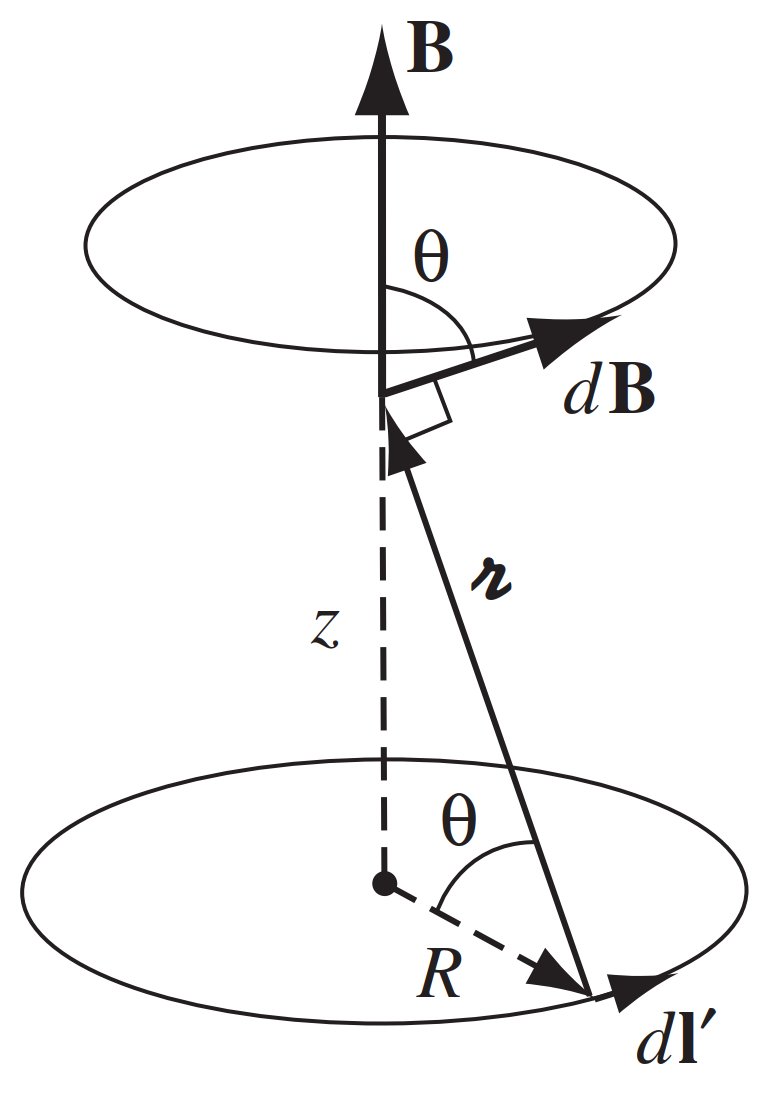
\includegraphics[height=0.3\textwidth]{../Rss/Electromagnetism/Magnetostatics/Loop.png}
\end{figure*}
We'll just jump straight to solving \textbf{B}
\begin{align*}
    \mathbf{B}&=\frac{\mu_0 I}{4\pi}\int \frac{d\mathbf{l}\times \brcurs}{|\rcurs^3|}\\
    \mathbf{B}&=\frac{\mu_0 I}{4\pi}\int \frac{(d s \;\mathbf{\hat{s}} +s \;d \phi \;\boldsymbol{\hat{\phi}}+  d z \;\mathbf{\hat{z}})\times (z\mathbf{\hat{z}}-s\mathbf{\hat{s}}-\phi\boldsymbol{\hat{\phi}})}{(R^2+z^2)^{3/2}}\\
    \mathbf{B}&=\frac{\mu_0 I}{4\pi}\int \frac{(z\;d \phi \;\mathbf{\hat{s}} +R^2  d \phi \;\mathbf{\hat{z}})}{{(R^2+z^2)}^{3/2}}\\
\end{align*}
Since the $\mathbf{\hat{s}}$ cancel itself, we only need to evaluate along $z$ axis
\begin{align*}
    \mathbf{B}&=\frac{\mu_0 I}{4\pi}\int \frac{R^2  d \phi \;\mathbf{\hat{z}}}{{R^2+z^2}^{3/2}}\\
    \mathbf{B}&=\frac{\mu_0 I}{2}\frac{R^2}{(R^2+z^2)^{3/2}}\mathbf{\hat{z}}
\end{align*}

\subsection*{Appendix III: Tugas 3 Listrik Magnet}
\subsubsection*{Soal 1.} Kawat lurus (cetak tebal) yang panjangnya L dialiri arus I. Dengan menggunakan hukum Biot-Savart, tentukanlah medan magnet yang terjadi di titik P, Q, R, dan S.
\begin{figure*}[ht]
    \centering
    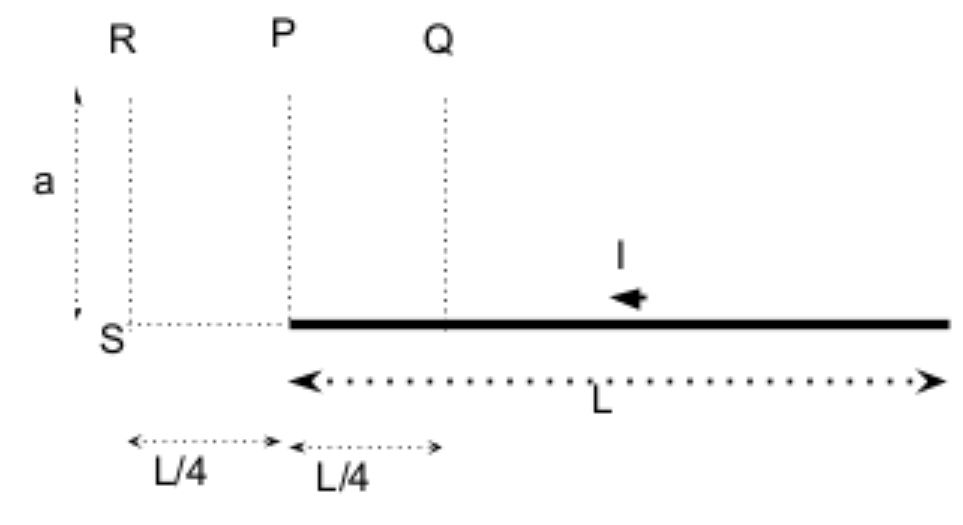
\includegraphics[width=0.5\textwidth]{../Rss/Electromagnetism/Magnetostatics/T3-1.PNG}
\end{figure*}

Medan magnet akan dievaluasi dalam koordinat tabung. Vektor pemisahan pada titik P, Q dan R adalah
\begin{equation*}
\brcurs(s,\phi,z)=s\mathbf{\hat{s}}+z\mathbf{\hat{z}}    
\end{equation*}
dengan magnitude 
\begin{equation*}
    |\rcurs|=(s^2+r^2)^{1/2}
\end{equation*}
Maka, medan magnet adalah 
\begin{align*}
    \mathbf{B}& =\frac{\mu_0 I}{4\pi}\int \frac{d\mathbf{l}\times \brcurs}{|\rcurs^3|}\\
    \mathbf{B}&=\frac{\mu_0 I}{4\pi}\int \frac{(d s \;\mathbf{\hat{s}} +s \;d \phi \;\boldsymbol{\hat{\phi}}+  d z \;\mathbf{\hat{z}})\times(s\mathbf{\hat{s}}+z\mathbf{\hat{z}})}{(s^2+r^2)^{3/2}}\\
\end{align*}
Karena integrasi dilakukan sepanjang sumbu $z$, maka $s, \phi$ adalah konstan dan $ds=d\phi=0$
\begin{align*}
    \mathbf{B}&=\frac{\mu_0 I}{4\pi}\int \frac{( dz \; \mathbf{\hat{z}}) \times (s\mathbf{\hat{s}}+z\mathbf{\hat{z}})}{(s^2+z^2)^{3/2}}\\
    \mathbf{B}&=\frac{\mu_0 I}{4\pi}\int \frac{s\;dz}{(s^2+z^2)^{3/2}}\boldsymbol{\hat{\phi}}
\end{align*}
dimana $\mathbf{\hat{z}}\times\mathbf{\hat{s}}=\boldsymbol{\hat{\phi}}$ dan $\mathbf{\hat{z}}\times\mathbf{\hat{z}}=0$. Kemudian diketahui titik P berjarak $a$ dari kawat, sehingga $s=a$ dan integral dihitung dari $z=0$ hingga $z=L$
\begin{align*}
    \mathbf{B}_P&=\frac{\mu_0 I}{4\pi}\int_{0}^{L} \frac{a\;dz}{(a^2+z^2)^{3/2}}\boldsymbol{\hat{\phi}}
\end{align*}
Integral dapat dievaluasi menggunakan subsitusi trigonometri atau hanya dengan melihat tabel, yang menghasilkan
\begin{align*}
    \mathbf{B}_P&=\frac{\mu_0 I}{4\pi}\frac{az}{a^2(a^2+z^2)^{1/2}}\bigg|_{0}^{L}\boldsymbol{\hat{\phi}}\\
    \mathbf{B}_P&=\frac{\mu_0 I}{4\pi a}\frac{L}{(a^2+L^2)^{1/2}}\boldsymbol{\hat{\phi}}
\end{align*}
Karena sumbu $z$ positif didefinisikan sesuai arah arus (ke kiri) maka, arah medah (positif $\boldsymbol{\hat{\phi}}$) adalah ke dalam bidang.

Pada titik Q, integral dihitung dari $z=-L/4$ hingga $z=L/3$. Maka 
\begin{align*}
    \mathbf{B}_Q&=\frac{\mu_0 I}{4\pi}\int_{-L/4}^{L/3} \frac{a\;dz}{(a^2+z^2)^{3/2}}\boldsymbol{\hat{\phi}}
\end{align*}
Seperti sebelumnya, integral dapat dievaluasi dengan subsitusi trigonometri atau tabel 
\begin{align*}
    \mathbf{B}_Q&=\frac{\mu_0 I}{4\pi}\frac{az}{a^2(a^2+z^2)^{1/2}}\bigg|_{-l/4}^{L/3}\boldsymbol{\hat{\phi}}\\
    \mathbf{B}_Q&=\frac{\mu_0 I}{4\pi a}\biggl( \frac{L/3}{(a^2+L^2/9)^{1/2}} + \frac{L/4}{(a^2+L^2/16)^{1/2}}\biggr)\boldsymbol{\hat{\phi}}
\end{align*}
Seperti sebelumnya, arah medan adalah ke dalam bidang.

Pada titik R, integral dihitung dari $z=L/4$ hingga $z=5L/4$. Maka 
\begin{align*}
    \mathbf{B}_R&=\frac{\mu_0 I}{4\pi}\int_{L/4}^{5L/4} \frac{a\;dz}{(a^2+z^2)^{3/2}}\boldsymbol{\hat{\phi}}\\
    \mathbf{B}_R&= \frac{\mu_0 I}{4\pi}\frac{az}{a^2(a^2+z^2)^{1/2}}\bigg|_{L/4}^{5L/4}\boldsymbol{\hat{\phi}}\\
    \mathbf{B}_R&=\frac{\mu_0 I}{4\pi a}\biggl( \frac{5L/4}{(a^2+25L^2/16)^{1/2}} - \frac{L/4}{(a^2+L^2/16)^{1/2}}\biggr)\boldsymbol{\hat{\phi}}
\end{align*}
Medan pada titik R berarah ke dalam bidang.

Pada titik S, medan adalah nol karena cross product dari vektor arah integrasi $d\mathbf{l}$ dengan vector pemisahan $\brcurs$ adalah nol. Diketahui vector pemisahan pada titik S 
\begin{equation*}    \brcurs(s,\phi,z)=z\mathbf{\hat{z}}    
\end{equation*}
dan vektor arah integrasi
\begin{equation*}
    d\mathbf{l}=d s \;\mathbf{\hat{s}} +s \;d \phi \;\boldsymbol{\hat{\phi}}+  d z \;\mathbf{\hat{z}}=dz \; \mathbf{\hat{z}}
\end{equation*}
karena $ds=d\phi=0$. Sehingga cross product kedua vector
\begin{equation*}
    d\mathbf{l}\times\brcurs= z\mathbf{\hat{z}}    \times dz \; \mathbf{\hat{z}}=0
\end{equation*}
mengingat $\mathbf{\hat{z}}\times\mathbf{\hat{z}}=0$. Hal ini menyebabkan medan pada S 
\begin{equation*}
    \mathbf{B}_S =\frac{\mu_0 I}{4\pi}\int \frac{d\mathbf{l}\times \brcurs}{|\rcurs^3|}=0
\end{equation*}
menjadi nol.

\subsubsection*{Soal 2.} Sebuah loop berbentuk lingkaran berjari-jari R dialiri arus listrik I. Dengan menggunakan hukum BiotSavart, tentukanlah :
\begin{itemize}
    \item Medan magnet di titik P.
    \item Medan magnet di pusat lingkaran loop.
\end{itemize}

\begin{figure*}[ht]
    \centering
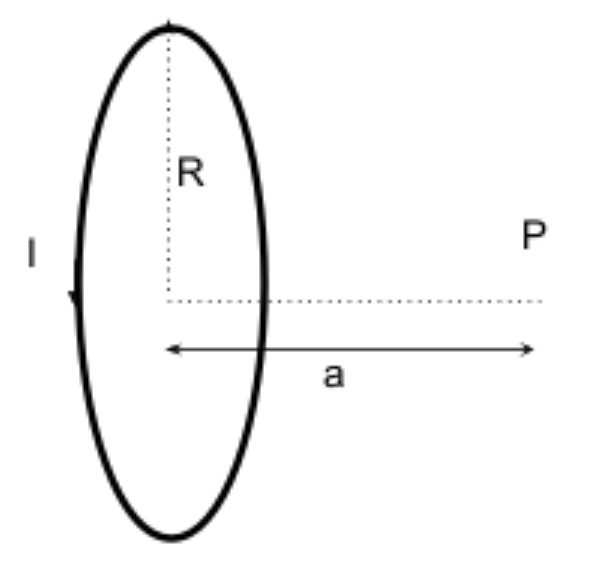
\includegraphics[width=0.3\textwidth]{../Rss/Electromagnetism/Magnetostatics/T3-2.PNG}
\end{figure*}

Medan akan dievaluasi dalam koordinat tabung. Selanjutnya sumbu $z$ didefinisikan sebagai arah dari pusat lingkaran ke titik P. Diketahui vektor pemisahan pada titik P sebagai 
\begin{equation*}
    \brcurs=a\mathbf{\hat{z}}-R\mathbf{\hat{s}}-\phi\boldsymbol{\hat{\phi}}
\end{equation*}
dengan magnitude
\begin{equation*}
    |\rcurs|=(R^2+z^2)^{1/2}
\end{equation*}
Maka, medan pada titik P 
\begin{align*}
    \mathbf{B}_P&=\frac{\mu_0 I}{4\pi}\int \frac{d\mathbf{l}\times \brcurs}{|\rcurs^3|}\\
    \mathbf{B}_P&=\frac{\mu_0 I}{4\pi}\int \frac{(d s \;\mathbf{\hat{s}} +R \;d \phi \;\boldsymbol{\hat{\phi}}+  d z \;\mathbf{\hat{z}})\times (a\mathbf{\hat{z}}-R\mathbf{\hat{s}}-\phi\boldsymbol{\hat{\phi}})}{(R^2+z^2)^{3/2}}\\
    \mathbf{B}_P&=\frac{\mu_0 I}{4\pi}\int \frac{ R \;d \phi \;\boldsymbol{\hat{\phi}}\times (a\mathbf{\hat{z}}-R\mathbf{\hat{s}}-\phi\boldsymbol{\hat{\phi}})}{(R^2+z^2)^{3/2}}\\
    \mathbf{B}_P&=\frac{\mu_0 I}{4\pi}\int \frac{(z\;d \phi \;\mathbf{\hat{s}} +R^2  d \phi \;\mathbf{\hat{z}})}{{(R^2+z^2)}^{3/2}}\\
\end{align*}
Karena komponen radial $\mathbf{\hat{s}}$ saling membatalkan, maka suku $z\;d \phi \;\mathbf{\hat{s}} $ dibuang. Kemudian integral dievaluasi dari $\phi=0$ hingga $\phi=2\pi$
\begin{align*}
    \mathbf{B}_P&=\frac{\mu_0 I}{4\pi}\int_{0}^{2\pi} \frac{R^2  d \phi \;\mathbf{\hat{z}}}{{(R^2+z^2)}^{3/2}}\\
    \mathbf{B}_P&=\frac{\mu_0 I}{2}\frac{R^2}{(R^2+z^2)^{3/2}}\mathbf{\hat{z}}
\end{align*}
Arah medan adalah ke kanan bidang (positif $z$).

Pada pusat lingkaran, $a=0$, sehingga
 \begin{equation*}
    \mathbf{B}_{\text{pusat}} =\frac{\mu_0 I}{2}\frac{R^2}{(R^2)^{3/2}}\mathbf{\hat{z}}=\frac{\mu_0 I}{2R}\mathbf{\hat{z}}
\end{equation*}
Arah medan adalah ke arah titik P (positif $z$).


\subsubsection*{Soal 3.} Suatu sistem terdiri atas kawat $\frac{3}{4}$ lingkaran dihubungkan dengan dua kawat lurus sejajar seperti gambar. Jika pada sistem mengalir arus I seperti gambar, tentukanlah medan magnet di titik P (pusat lingkaran).
\begin{figure*}[ht]
    \centering
    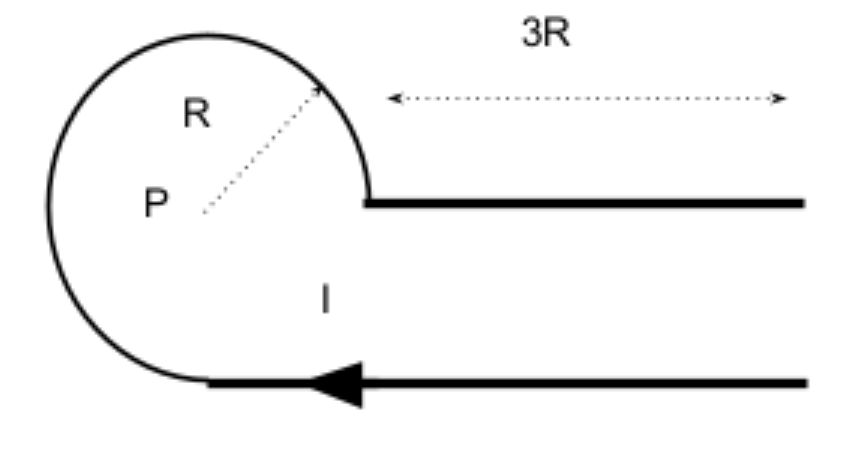
\includegraphics[width=0.5\textwidth]{../Rss/Electromagnetism/Magnetostatics/T3-3.PNG}
\end{figure*}

Medan pada pusat lingkaran P merupakan superposisi dari 3 medan yang diakibatkan oleh tiga kawat: kawat lurus 3R, kawat melingkar $\frac{3}{2}\pi R$ dan kawat lurus 4R.

Medan akibat kawat lurus 3R adalah nol karena titik P paralel dengan arah arus, seperti pada soal pertama bagian titik S
\begin{equation*}
    \mathbf{B}_1=0
\end{equation*}

Medan akibat kawat melingkar adalah
\begin{align*}
    \mathbf{B}_2&=\frac{\mu_0 I}{4\pi}\int \frac{R^2  d \phi \;\mathbf{\hat{z}}}{{R^2+z^2}^{3/2}}\\
\end{align*}
Karena lingkaran melingkar sepanjang $\frac{3}{2}\pi R$, integrasi dilakukan sepanjang $\phi=0$ hingga $\phi=\frac{3}{2}\pi $
\begin{align*}
    \mathbf{B}_2&=\frac{\mu_0 I}{4\pi}\int_{0}^{\frac{3}{2}\pi} \frac{R^2  d \phi \;\mathbf{\hat{z}}}{{R^2+z^2}^{3/2}}\\
    \mathbf{B}_2&=\frac{3\mu_0 I}{8}\frac{R^2}{(R^2+z^2)^{3/2}}\mathbf{\hat{z}}
\end{align*}
dimana positif $z$ didefinisikan ke arah dalam bidang. Karena titik P berada pada pusat lingkaran maka $z=0$ 
\begin{equation*}
    \mathbf{B}_2=\frac{\mu_0 I}{2}\frac{R^2}{(R^2)^{3/2}}\mathbf{\hat{z}}=\frac{\mu_0 I}{2R}\mathbf{\hat{z}}
\end{equation*}

Medan akibat kawat lurus adalah
\begin{equation*}
    \mathbf{B} =\frac{\mu_0 I}{4\pi}\int \frac{s\;dz}{(s^2+z^2)^{3/2}}\boldsymbol{\hat{\phi}}
\end{equation*}
Karena kawat membentang sepanjang $4R$, maka integrasi dilakukan dari $z=0$ hingga $z= 4R$. Perlu dicatat bahwa sumbu $z$ yang didefinisikan pada kawat lurus tidak sama dengan sumbu $z$ pada kawat melingkar. Namun, arah medan kedua medan adalah sama: ke dalam bidang. Kembali ke pengevaluasian medan 
\begin{align*}
    \mathbf{B}_3 &=\frac{\mu_0 I}{4\pi}\int_{0}^{4R} \frac{R\;dz}{(R^2+z^2)^{3/2}}\boldsymbol{\hat{\phi}}\\
    \mathbf{B}_3&=\frac{\mu_0 I}{4\pi}\frac{Rz}{R^2(R^2+z^2)^{1/2}}\bigg|_{0}^{4R}\boldsymbol{\hat{\phi}}\\
    \mathbf{B}_3&=\frac{\mu_0 I}{4\pi R}\frac{4R}{(R^2+16R^2)^{1/2}}\boldsymbol{\hat{\phi}}\\
    \mathbf{B}_3&=\frac{\mu_0 I\sqrt{17}}{17\pi R} \boldsymbol{\hat{\phi}}
\end{align*}
dengan arah ke dalam bidang. Karena arah ke dalam bidang sebelumnya didefinisikan sebagai sumbu $z$ maka medan dapat ditulis
\begin{equation*}
    \mathbf{B}_3=\frac{\mu_0 I\sqrt{17}}{17\pi R} \mathbf{\hat{z}}
\end{equation*}

Selanjutnya, medan pada titik P merupakan resultan dari ketiga medan yang telah dievaluasi
\begin{align*}
    \sum \mathbf{B}& =\mathbf{B}_1+\mathbf{B}_2+\mathbf{B}_3\\
    \sum \mathbf{B}& =\frac{\mu_0 I}{2R}\mathbf{\hat{z}}+\frac{\mu_0 I\sqrt{17}}{17\pi R} \mathbf{\hat{z}}\\
    \sum \mathbf{B}& =\frac{\mu_0 I}{R}\biggl(\frac{1}{2}+\frac{\sqrt{17}}{17\pi}\biggr)\mathbf{\hat{z}}
\end{align*}
dengan arah ke dalam bidang.

\subsection*{Appendix IV: Ampere's Law}
\subsubsection*{Infinite straight lines.} Find the magnetic field a distance $s$ from a long straight wire carrying a steady current $I$, This is the same problem we solved using the Biot-Savart's Law. 

We know the direction of \textbf{B} is “circumferential,” circling around the wire as indicated by the right-hand rule. By symmetry, the magnitude of \textbf{B} is constant around an Amperian loop of radius $s$, centered on the wire. So Ampère’s law gives
\begin{align*}
    \oint \mathbf{B}\cdot d\mathbf{l}&=\mu_0I_{\text{enc}}\\
    B2\pi s&=\mu_0I\\
    B&=\frac{\mu_0I}{2\pi s}
\end{align*}
Since we know the direction of \textbf{B} is “circumferential,” we can write the expression as 
\begin{equation*}
    \mathbf{B}=\frac{\mu_0I}{2\pi s}\boldsymbol{\hat{\phi}}
\end{equation*}
\begin{figure*}[ht]
    \centering
    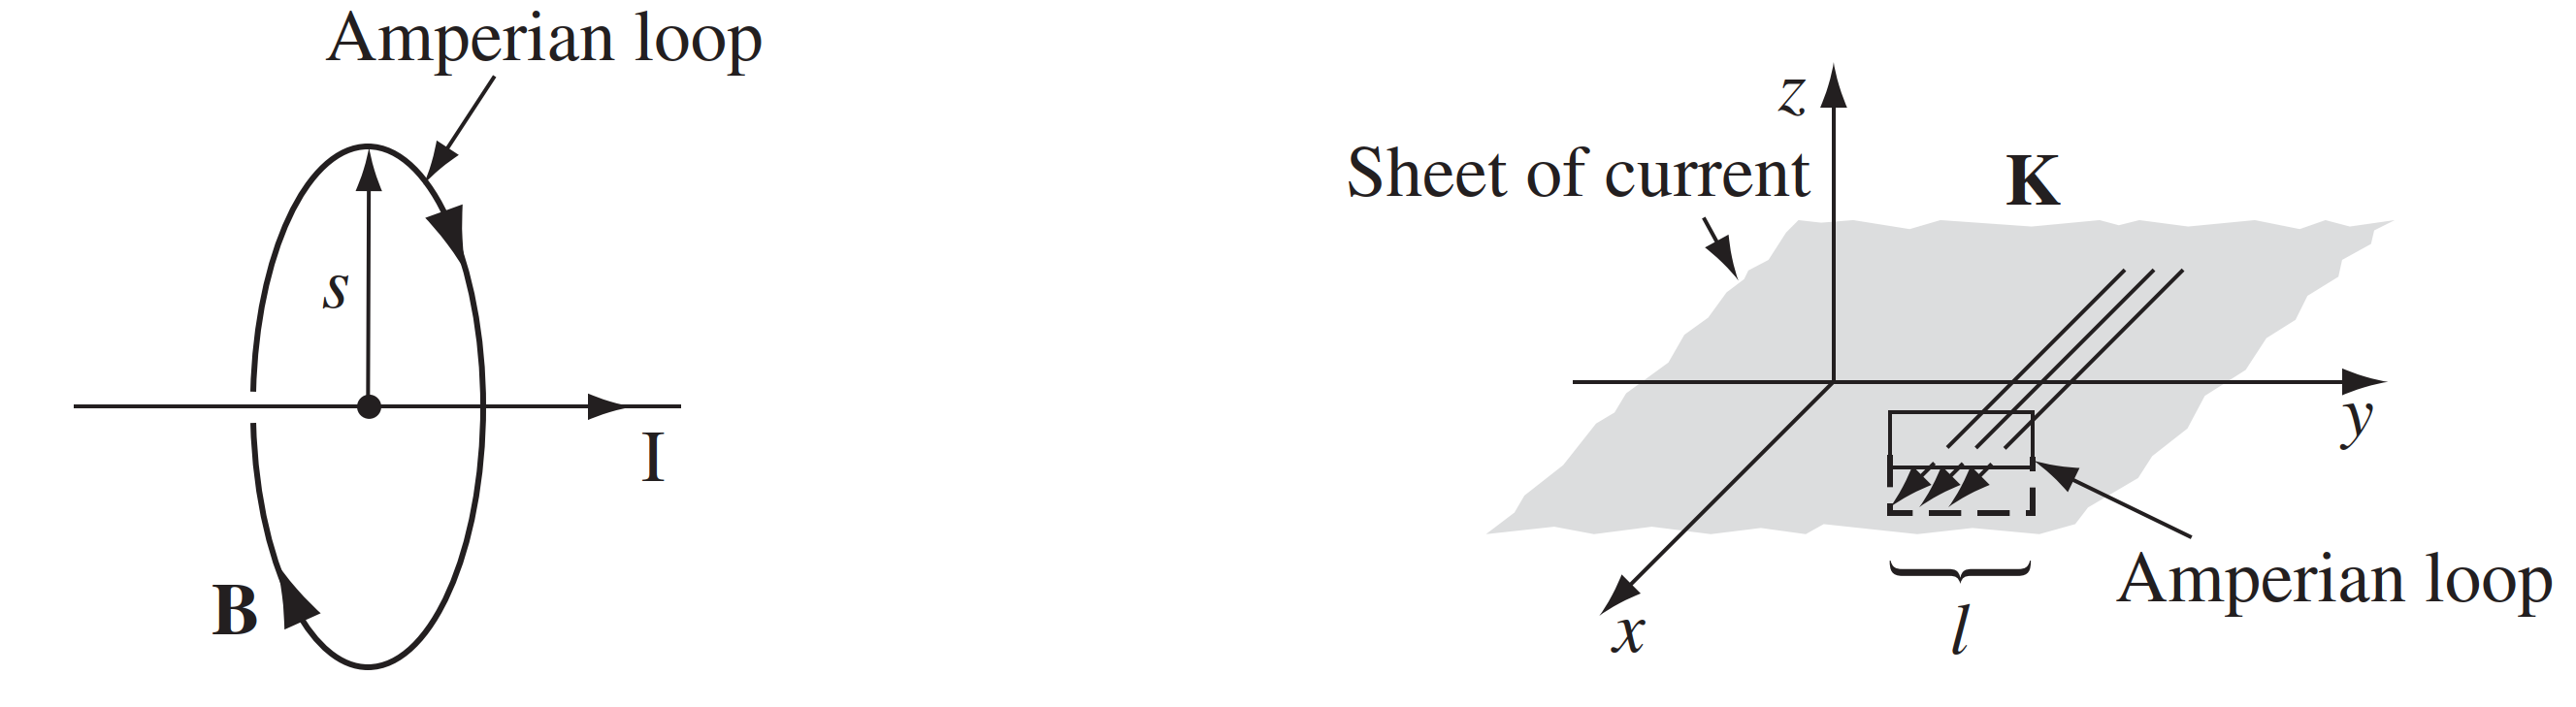
\includegraphics[width=0.8\textwidth]{../Rss/Electromagnetism/Magnetostatics/Ampere-1.png}
\end{figure*}

\subsubsection*{Infinite planes.} Find the magnetic field of an infinite uniform surface current 
$\mathbf{K} = K \mathbf{\hat{x}}$, flowing over the $xy$ plane. 

\textbf{B} can only have a y component, and a quick check with your right hand should convince you that it points to the left above the plane and to the right below it. With this in mind, we draw a rectangular Amperian loop parallel to the $yz$ plane and extending an equal distance above and below the 
surface. Applying Ampère’s law,
\begin{align*}
    \oint \mathbf{B}\cdot d\mathbf{l}&=\mu_0I_{\text{enc}}\\
    2Bl&=\mu_0Kl\\
    B&=\frac{\mu_0}{2}K
\end{align*}
or, more precisely
\begin{equation*}
    \mathbf{B}=
    \begin{cases}
        \dfrac{\mu_0}{2}K\;\mathbf{\hat{y}},&z<0\\
        -\dfrac{\mu_0}{2}K\;\mathbf{\hat{y}},&z>0\\
    \end{cases}
\end{equation*}

\subsubsection*{Infinite solenoids.} Find the magnetic field of a very long solenoid, consisting of $n$ closely wound turns per unit length on a cylinder of radius $R$, each carrying a steady current $I$.

\begin{figure*}[ht]
    \centering
    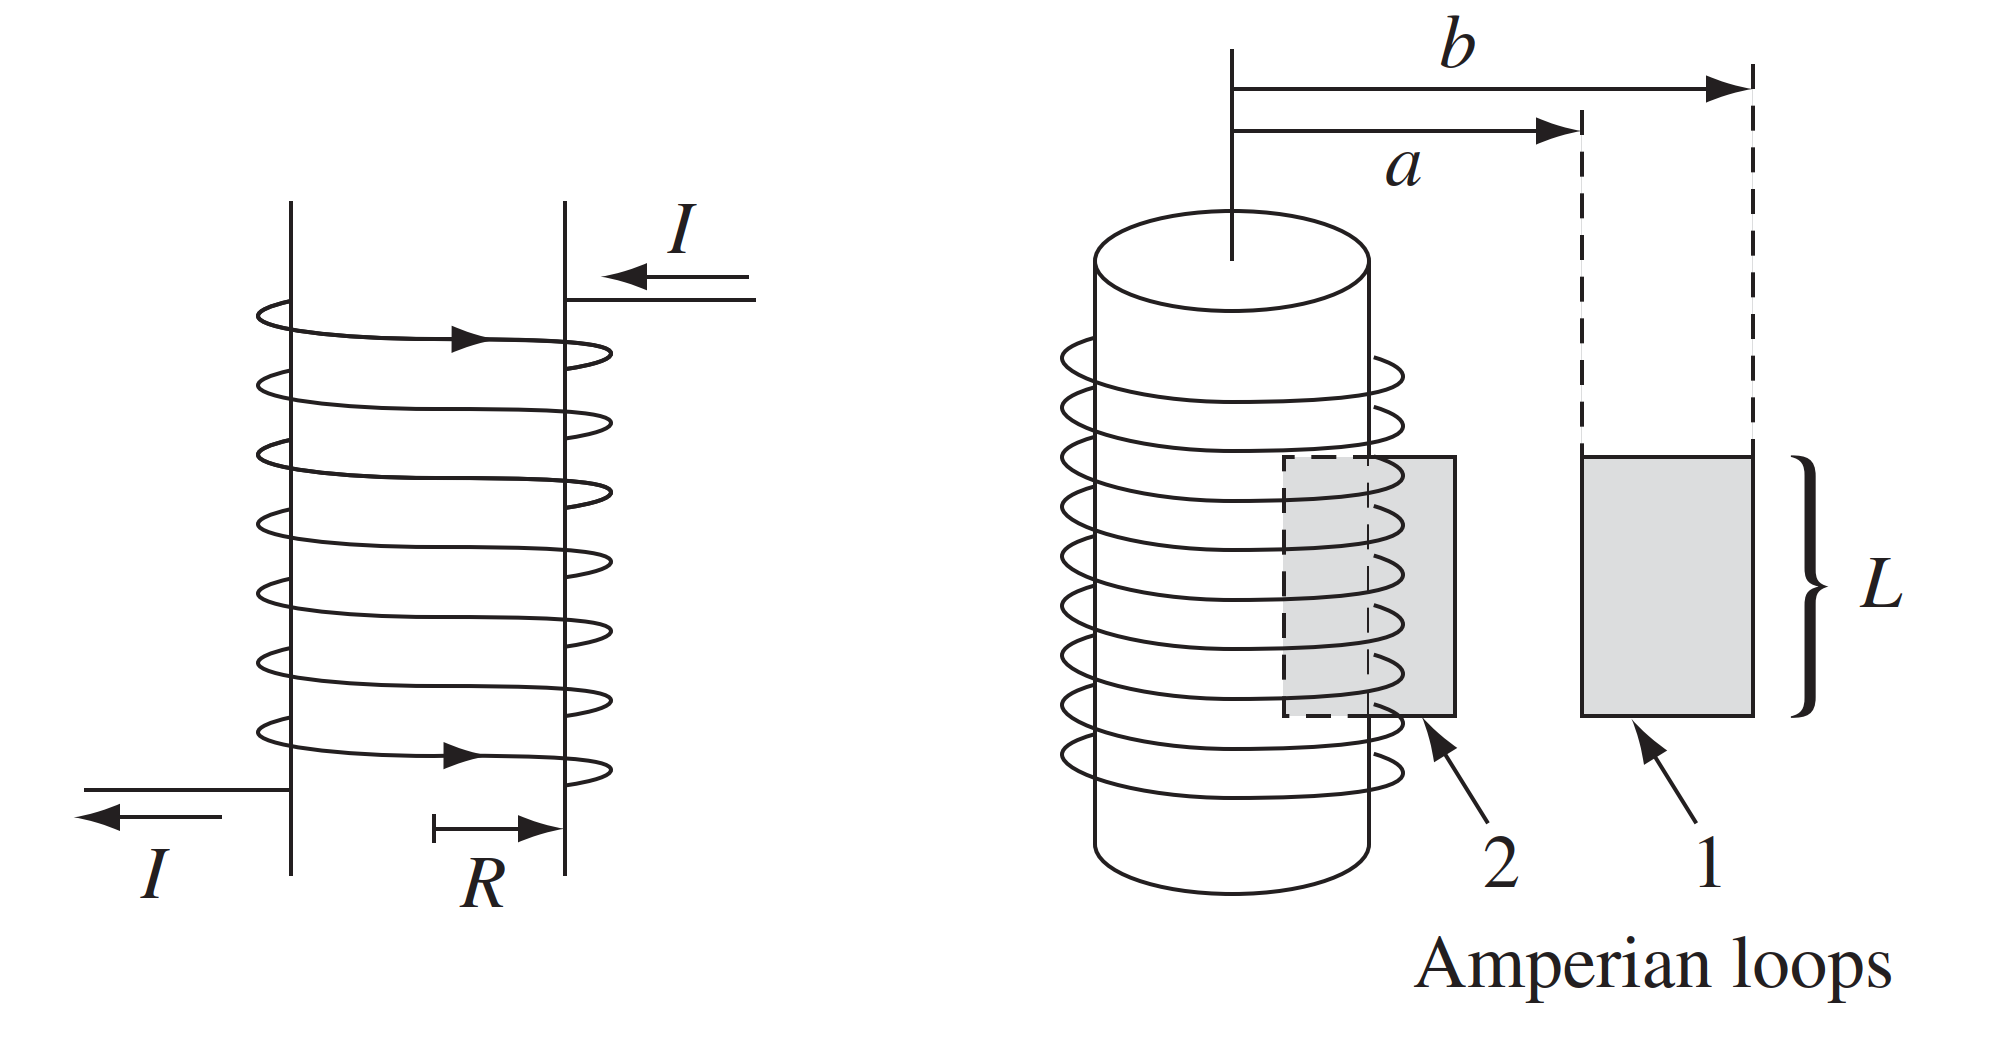
\includegraphics[width=0.75\textwidth]{../Rss/Electromagnetism/Magnetostatics/Solenoid.png}
\end{figure*}

Magnetic field of an infinite, closely wound solenoid runs parallel to the axis. From the right-hand rule, we expect that it points upward inside the solenoid and downward outside. Moreover, it certainly approaches zero as you go very far away. With this in mind, let’s apply Ampère’s law to the two rectangular loops. Loop 1 lies entirely outside the solenoid, with its sides at distances $a$ 
and $b$ from the axis
\begin{align*}
    \oint \mathbf{B}\cdot d\mathbf{l}&=\mu_0I_{\text{enc}}\\
    [B(a)-B(b)]l&=0\\
\end{align*}
so 
\begin{equation*}
    B(a)=B(b)
\end{equation*}
Evidently the field outside does not depend on the distance from the axis. But we agreed that it goes to zero for large $s$. It must therefore be zero everywhere! As for loop 2, which is half inside and half outside, Ampère’s law gives
\begin{align*}
    \oint \mathbf{B}\cdot d\mathbf{l}&=\mu_0I_{\text{enc}}\\
    BL&=\mu_0nIL
\end{align*}
where B is the field inside the solenoid. The right side of the loop contributes 
nothing, since B = 0 out there. Conclusion
\begin{equation*}
    \mathbf{B}=\begin{cases}
        \mu_0nIL\;\mathbf{\hat{z}}&\text{inside solenoid}\\
        0&\text{outside solenoid}
    \end{cases}
\end{equation*}

\subsubsection*{Toroid.} A toroidal coil consists of a circular ring, or “donut,” around which a long wire is wrapped. The winding is uniform and tight enough so that each turn can be considered a plane closed loop. The cross-sectional shape of the coil is immaterial. In that case, it follows that the magnetic field of the toroid is circumferential at all points, both inside and outside the coil. I will first determine the direction of the field using Biot-Savart, then I will determine the magnitude using Ampere's Law.

\begin{figure*}
    \centering
    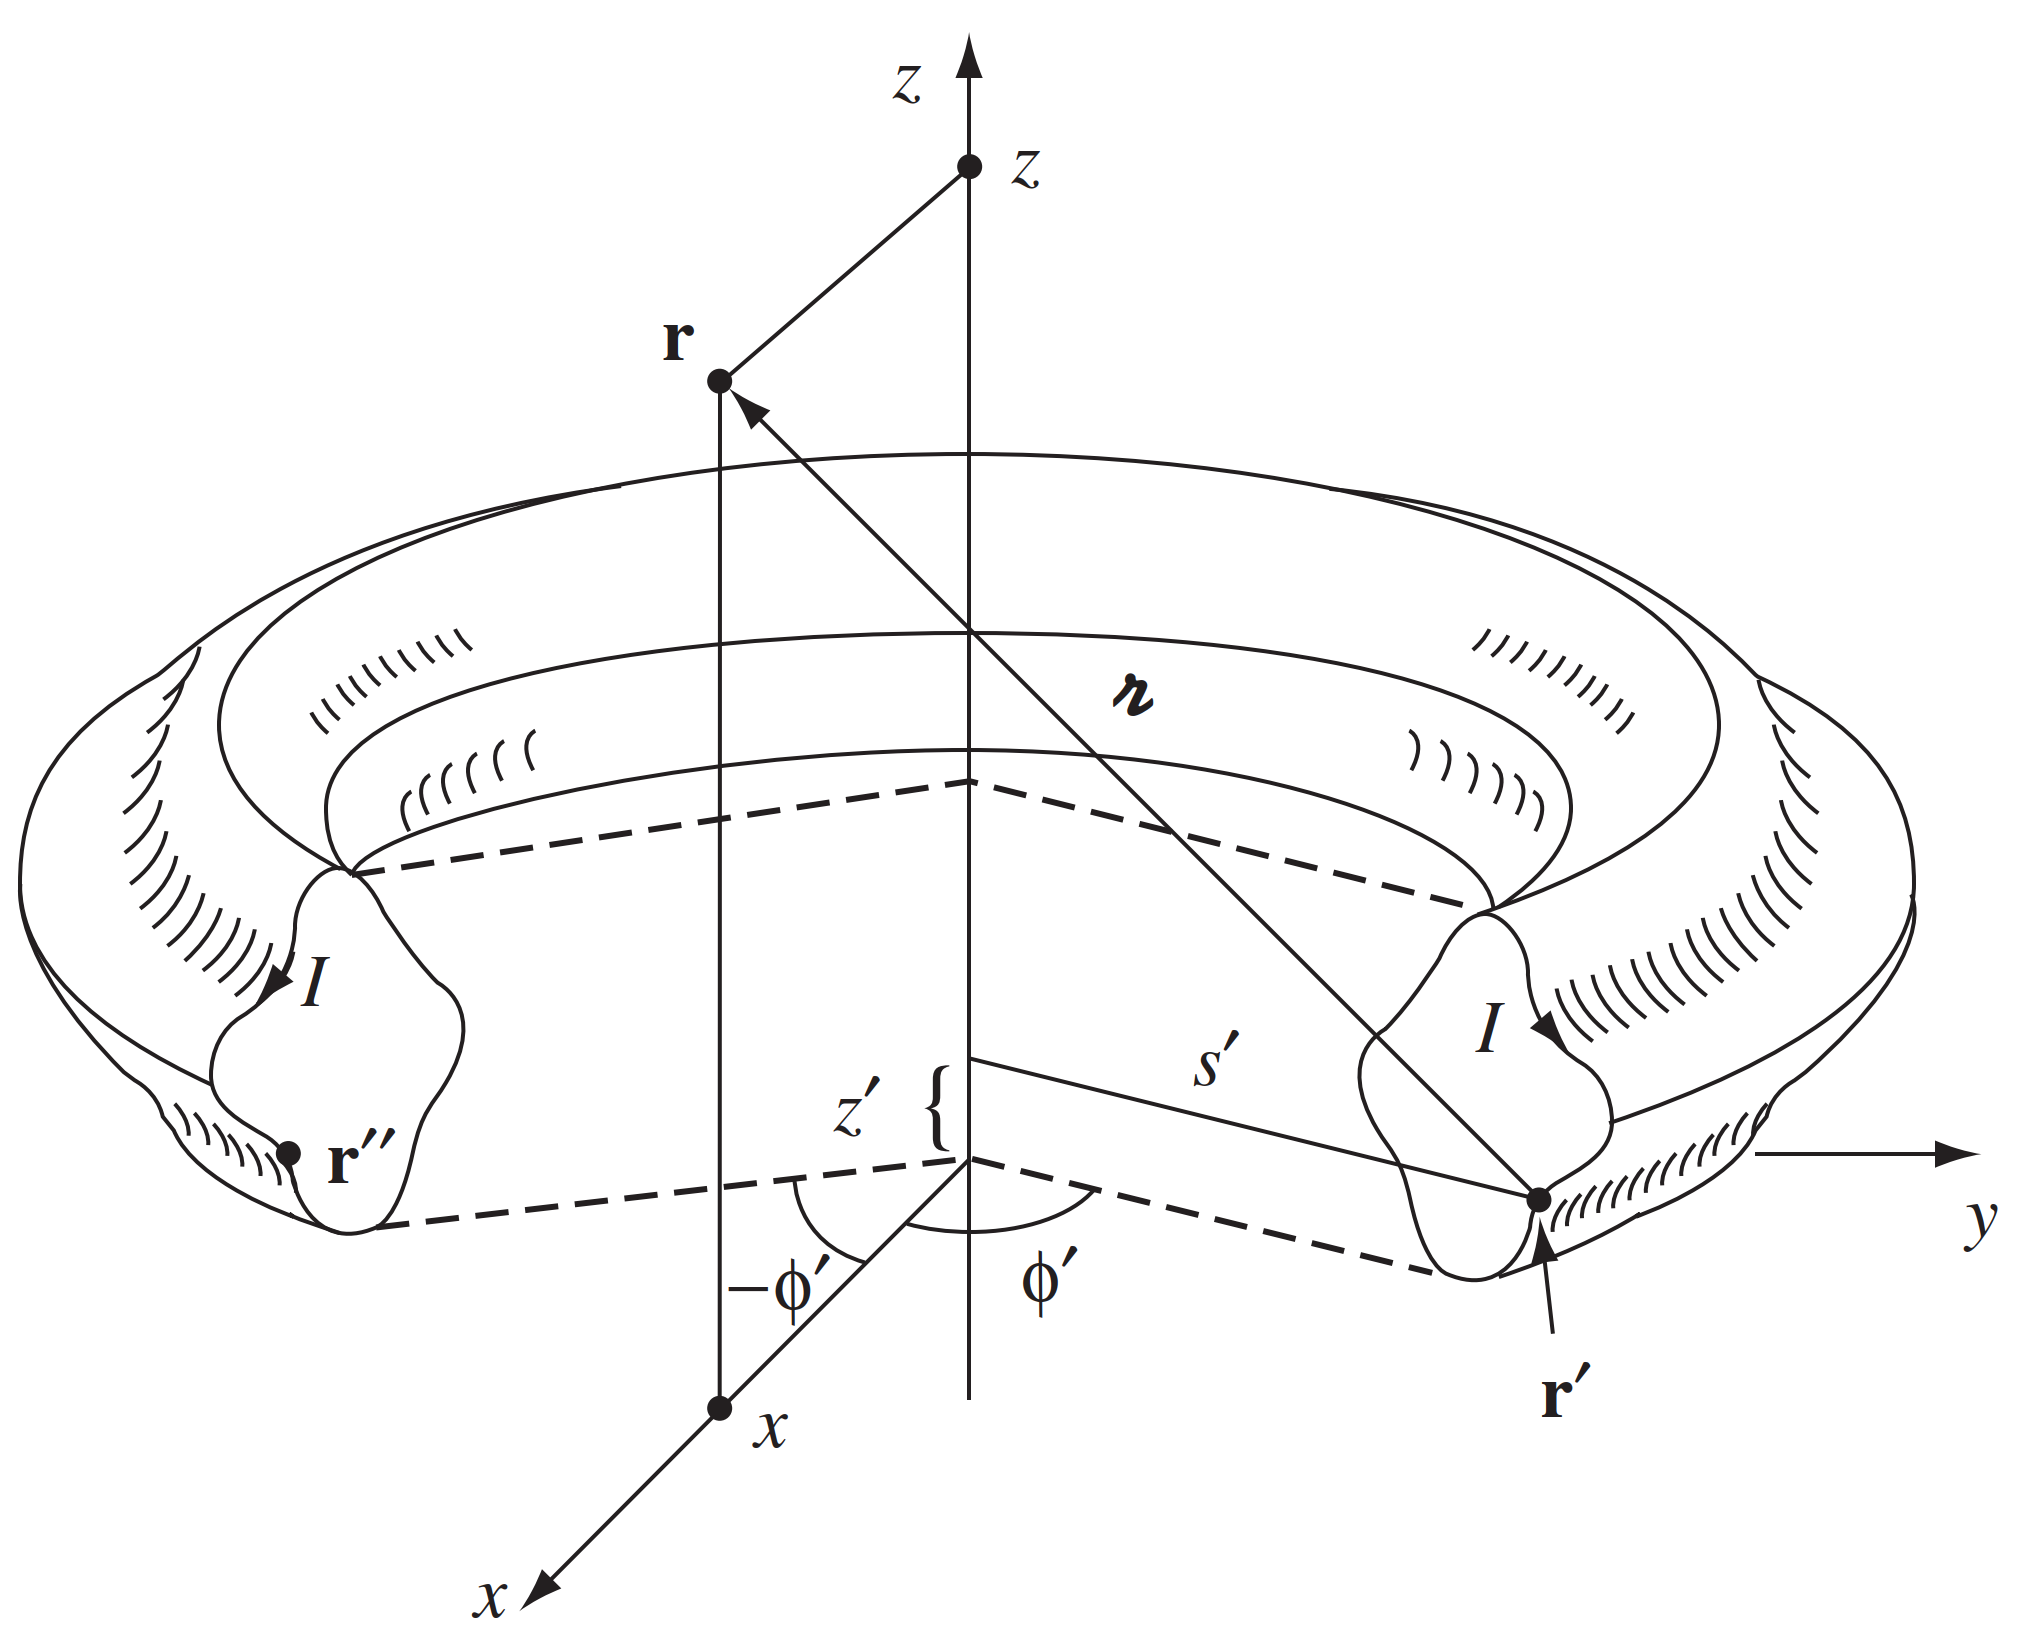
\includegraphics[width=0.75\textwidth]{../Rss/Electromagnetism/Magnetostatics/Toroid.png}
\end{figure*}

First the direction. According to the Biot-Savart law, the field at \textbf{r} due to the current at \textbf{r'} is 
\begin{equation*}
    \mathbf{B}(\mathbf{r})=\frac{\mu_0}{4\pi}\int \frac{\mathbf{I}\times\brcurs}{\rcurs^3}dl'
\end{equation*}
The separation vector is 
\begin{align*}
    \brcurs&=(s\mathbf{\hat{s}}+\phi\boldsymbol{\hat{\phi}}+z\mathbf{\hat{z}})-(s'\mathbf{\hat{s}}+\phi'\boldsymbol{\hat{\phi}}+z'\mathbf{\hat{z}})\\
    &=(s-s')\mathbf{\hat{s}}+ (\phi-\phi')\boldsymbol{\hat{\phi}}+(z-z')\mathbf{\hat{z}}
\end{align*}
Then, since the current has no $\phi$ component
\begin{equation*}
    \mathbf{I}=I = I_s \mathbf{\hat{s}} + I_z \mathbf{\hat{z}}
\end{equation*}
Accordingly
\begin{align*}
    \mathbf{I}\times\brcurs&=
    \begin{vmatrix}
        \mathbf{\hat{s}}&\boldsymbol{\hat{\phi}}&\mathbf{\hat{z}}\\
        I_s&0&I_z\\
        s-s'&\phi-\phi'&z-z'\\
    \end{vmatrix}\\
    &=I_z(\phi'-\phi)\mathbf{\hat{s}}+\big[I_z(s-s')-I_s(\phi-\phi')\big]\boldsymbol{\hat{\phi}}+I_s(\phi-\phi')\mathbf{\hat{z}}\\
    &=I_z(s-s')\boldsymbol{\hat{\phi}}
\end{align*}
where the last line is evaluated due to symmetry. The symmetry in question situated at $r''$, with the same $s'$, the same $r$, the same $dl''$, the same $I_s$, and the same $I_z$, but negative $\phi'$. Because $\psi'$ changes sign, the $ \mathbf{\hat{s}}$ and $ \mathbf{\hat{z}}$ leaving only a $\boldsymbol{\hat{\phi}}$ term. Thus, the field is circumferential. $\blacksquare$

Now that we know the field is circumferential, determining its magnitude is ridiculously easy. Just apply Ampère’s law to a circle of radius $s$ about the axis of the toroid:
\begin{align*}
    \oint \mathbf{B}\cdot d\mathbf{l}&=\mu_0I_{\text{enc}}\\
    B2\pi s&=\mu_0NI
\end{align*}
where $N$ is the total number of turns. And hence
\begin{equation*}
    \mathbf{B}=\begin{cases}
        \dfrac{\mu_0NI}{2\pi s}&\text{for points inside the coil}\\
        0&\text{for points outside the coil}
    \end{cases}
\end{equation*}

\end{document}